% Manuscript prepared for submission to Empirical Software Engineering
% (Springer). Per EMSE's own submission guidelines
% (https://link.springer.com/journal/10664/submission-guidelines), no
% specific camera-ready LaTeX template is required at initial submission:
% "the compiled PDF will be used for peer-review purposes"; production
% reformats accepted manuscripts. This file therefore uses a generic
% article class but follows EMSE's required content structure: title page
% fields, a 150-250 word (optionally structured) abstract, 4-6 keywords,
% author-year in-text citations with an alphabetized DOI-linked reference
% list, an explicit LLM/AI-use disclosure, a Threats to Validity section,
% and a closing Statements and Declarations section.
\documentclass[11pt]{article}
\usepackage[margin=1in]{geometry}
\usepackage{graphicx}
\usepackage{booktabs}
\usepackage{amsmath}
\usepackage[hidelinks]{hyperref}
\usepackage{xcolor}
\usepackage{microtype}
\usepackage[round,authoryear]{natbib}

\title{The Notebook You Read Is Not the Notebook That Ran:\\
Execution-Order Reconstruction for LLM Understanding of Jupyter Notebooks}

% --- Title page fields (EMSE requires: author name(s), affiliation(s),
% corresponding-author email, ORCID if available). Affiliation confirmed by
% the author (Department of Computer Science and Engineering, Rajshahi
% University of Engineering and Technology, Rajshahi, Bangladesh); no ORCID
% will be used. Corresponding-author email confirmed by the author
% (raiyanrohit10@gmail.com).
\author{MD.\ Raiyan Bin Rafique \\
\textit{Department of Computer Science and Engineering} \\
\textit{Rajshahi University of Engineering and Technology, Rajshahi, Bangladesh} \\
Corresponding author: \texttt{raiyanrohit10@gmail.com}}
\date{}

\begin{document}
\maketitle

\begin{abstract}
\noindent\textbf{Context:} A Jupyter notebook stores cells in \emph{visual}
order, which often differs from the \emph{execution} order they actually
ran in. Its JSON format also buries code under base64 images, duplicate
MIME formats, and metadata. Stripping content saves tokens but also loses
clues needed to recover true execution order.
\textbf{Objective:} We test whether reconstructing execution order
improves an LLM's ability to track program state, both in controlled and
real settings.
\textbf{Method:} We built JupPreprocessor, a serializer that never calls
an LLM: it resolves what it can recover statically and flags what it
cannot. We evaluated it on a synthetic benchmark spanning fifteen models
and seven vendors, and on ground truth from re-executing 112 real
crashed notebooks (JunoBench) under both orderings.
\textbf{Results:} Unaided, models resolve state correctly 0\%--97\% of the
time; our fix scores 100\% at roughly 95\% fewer tokens.
On 52 real order-divergent variables, however, our serializer shows no
per-item accuracy advantage over the raw file for gpt-4o, our one answer
model on this corpus, once it answers (23--27\% correct, overlapping
95\% confidence intervals), a result that held after we fixed a grading
bug. The defensible advantage is narrower: the raw file is too large to fit
in context for 62\% of these items, versus 15--17\% for the compressed
formats.
\textbf{Conclusions:} Execution-order reconstruction is necessary and
sufficient for state-tracking in a controlled setting. On real notebooks,
our evidence shows only that the serializer keeps more notebooks
readable, not that answers become more accurate once a file is readable.
\end{abstract}

\noindent\textbf{Keywords:} Jupyter notebooks; large language models;
execution-order reconstruction; program state serialization; empirical
software engineering; notebook reproducibility

\section{Introduction}
Ask a large language model to debug a Jupyter notebook, and it will
confidently reason about a version of events that may never have
happened. This is because the \texttt{.ipynb} file format records cells
in the order they visually appear on screen, not the order they were
actually executed in. A user can run cell three, then cell one, then
delete cell two entirely, and the saved file will still list the cells
top to bottom as if nothing unusual occurred. The only surviving trace of
what really happened is a small integer attached to each cell, called
\texttt{execution\_count}, which simply records the number of times the
notebook's kernel has executed something by the time that cell last ran.
As we show later in this paper, models frequently fail to use this signal
correctly even when it is sitting right there in the file
(Sect.~\ref{sec:niah}).

This is not a rare edge case. A prior large-scale study of GitHub
notebooks found that roughly 36\% of them execute their cells in a
non-linear order \citep{siddik2025}. We wanted to know how bad the
problem is specifically for the population an LLM assistant is most
likely to encounter: notebooks that were saved right after a crash, where
a user was actively debugging something and did not have time to clean
up. We found the picture is considerably worse than the general GitHub
average: \textbf{59.8\% of these notebooks are saved out of order, 89.3\%
show gaps consistent with cells being re-run or deleted, and 92.0\% carry
at least one of these warning signs} (Sect.~\ref{sec:scan}).

We organize our empirical investigation around five research questions,
each answered in a specific part of the paper rather than left implicit:
\begin{itemize}
  \item \textbf{RQ1.} How prevalent are non-linear execution and other
        state hazards in real, crashed machine-learning notebooks, the
        population most likely to be handed to an LLM for debugging?
        (Sect.~\ref{sec:scan})
  \item \textbf{RQ2.} Does execution-order reconstruction measurably
        improve LLM state-tracking accuracy on a fair, context-bounded
        synthetic benchmark, isolated from mere retrieval-under-noise
        and from token-count confounds? (Sect.~\ref{sec:niah})
  \item \textbf{RQ3.} Does this synthetic-benchmark advantage transfer
        to real, messy notebooks, when measured against executable
        ground truth rather than assumed correctness?
        (Sect.~\ref{sec:realnb}--\ref{sec:judgeaudit})
  \item \textbf{RQ4.} What is the token-cost and robustness profile of
        the preprocessing pipeline on real notebooks, and does adding
        state-safety annotations erode the token savings? (Sect.~5.1)
  \item \textbf{RQ5.} Where does the approach fail or reach its limits,
        on already-clean data, in the preprocessor's own core
        execution-order-sort mechanism, and relative to alternative
        architectures such as reactive notebooks?
        (Sect.~\ref{sec:honestneg}, Sect.~\ref{sec:threats}, Sect.~7)
\end{itemize}

Answering these five questions is also how this paper makes its four
main contributions:
\begin{enumerate}
  \item \textbf{A three-tier treatment framework.} We separate what a
        preprocessing tool can actually \emph{resolve} on its own from
        what it can only \emph{detect and flag} because the true value
        was simply never written down anywhere in the file, and from what
        genuinely requires \emph{running the code} to know for certain.
  \item \textbf{JupPreprocessor}, an implementation of the first two
        tiers that never calls an LLM and never executes any code itself.
        It adds six lightweight annotations to a notebook (a history of
        how each variable was mutated over time, the last value a deleted
        ``ghost'' variable was seen holding, a flag for code whose output
        may not be reproducible, whether an error was later worked around
        or was fatal, inferred type and shape information, and a flag for
        a specific weakness in its own ordering logic that we discovered
        and describe below, affecting 26.6\% of real notebooks). All six
        together cost well under 1\% in extra tokens.
  \item \textbf{A fair benchmark we call Notebook-NIAH.} It is built so
        that the baseline condition always fits inside the model's
        context window; running out of room is recorded as its own
        outcome, never scored as a wrong answer. It includes a
        compression-only control, a comparison between a ``static'' task
        (plain retrieval) and a ``stateful'' task (state reconstruction) to
        separate the two skills, component-by-component ablations, and a
        capability curve spanning fifteen models across seven vendors.
  \item \textbf{Executable ground truth on real notebooks.} By actually
        re-running out-of-order notebooks under both their visual and
        their true execution order, we surface real variables whose final
        value differs between the two readings, in effect showing that
        the model a user thinks they trained is not always the model they
        actually trained. This gives us the first real-notebook
        state-accuracy measurement of its kind, together with an honest
        account of what still does not work.
\end{enumerate}
To our knowledge, this is the first paper to treat notebook serialization
format itself as a controlled experimental variable, holding the answer
model and prompt fixed and varying only how the notebook is encoded,
and to evaluate that variable specifically on crashed, out-of-order
notebooks rather than the cleaner, curated corpora used elsewhere in this
literature (Sect.~\ref{sec:relwork} contrasts this directly against the
closest prior systems).

\section{Root Causes and the Coupling Problem}
\label{sec:causes}
We group the problems that make a \texttt{.ipynb} file hard for an LLM to
understand into ten root causes, six about program state and four about
token cost. The state causes are: (A) non-linear execution, meaning the
saved order does not match the run order; (B) in-place mutation, where an
operation changes an object without leaving any static trace of the
change; (C) ghost variables, names that are still referenced later in the
notebook even though the cell that created them was deleted; (D)
re-execution divergence, where re-running a cell with a different random
seed, a changed input file, or a live network call would produce a
different result than what is stored; (E) silenced errors, where a
traceback is visible but a later cell shows the user worked around it
successfully; and (F) type erasure, where an output is stored as plain
text and the reader can no longer tell whether it represents a number, a
table, or an image description. The token causes are: (G) the same output
being duplicated across several MIME formats (for example, a table stored
simultaneously as plain text, HTML, and LaTeX); (H) images encoded as
long base64 text strings that a model cannot see but must still pay to
read as tokens; (I) old outputs from earlier runs of a cell being kept
alongside the current one; and (J) the sheer verbosity of nested JSON
structure itself. These two groups pull against each other: restoring
missing state information costs tokens, and cutting tokens tends to
remove exactly the state information a model would need.

Three of the six state causes cannot be solved by any amount of clever
static analysis, because the information they concern was never written
into the file in the first place. A cell that mutates an object in place
(B) leaves no record of what the object looked like afterward. A deleted
cell that created a ghost variable (C) leaves no record of what created
it. A cell that behaves differently on re-execution (D) leaves no record
of what the alternative outcome would have been. Table~\ref{tab:tiers}
turns this observation into a concrete design rule: our tool should not
pretend to have solved something it cannot actually know. The key idea
behind our second tier is that a model does not need the missing value in
order to avoid a wrong answer; it only needs to know that the value is
missing, and roughly where the uncertainty entered the notebook. Once a
model is told ``this could be wrong,'' it reasons more carefully than it
would given no warning at all.

\begin{table}[t]
\centering\small
\begin{tabular}{@{}lllp{6.2cm}@{}}
\toprule
Tier & Treatment & Causes & Mechanism \\
\midrule
1 & Resolve & A, G--J & Reorder by \texttt{execution\_count}; strip
MIME/base64/metadata; latest output only; YAML \\
2 & Detect \& flag & B--F & Mutation timeline; ghost last-observed value;
divergence-risk flags; tolerated/terminal errors; typed shape hints \\
3 & Runtime verify & B--E fully & Sandboxed re-execution diffed against static
predictions \\
\bottomrule
\end{tabular}
\caption{The three-tier treatment framework.}
\label{tab:tiers}
\end{table}

\section{JupPreprocessor}
\label{sec:method}
JupPreprocessor is a single-pass, deterministic transform written in
Python. It never calls an LLM, never makes a network request, and never
attaches to a Python kernel; it only reads the static text of the
notebook file. Given a raw \texttt{.ipynb} file, it produces a YAML
document containing an \texttt{execution\_order} field that lists the
cells in the order they were actually run, not the order they
appear on screen, with markdown cells re-attached to whichever code cell
they originally preceded. Each cell is annotated with an
\texttt{error\_status} (was any error tolerated or fatal) and a
\texttt{divergence\_risk} flag (does this cell contain code, such as an
unseeded random draw or a network call, whose output might change on
re-execution). Alongside the cells, the tool produces a
\texttt{variables} table recording, for every name it can track: its
inferred type, its shape where one can be inferred, the cell that first
defined it, the cell that most recently touched it, a short history of
how it was mutated, a status of either \texttt{active} or \texttt{ghost},
and a confidence level for all of the above. If a cell contains something
the Python parser cannot handle on its own, such as an IPython magic
command or a shell escape, the tool falls back to a simpler regular
expression parser for that cell rather than giving up on the notebook
entirely. We chose YAML over the notebook's native JSON purely for
compactness: the same structural information costs noticeably fewer
tokens once repeated key names and bracket nesting are removed.

Sorting by \texttt{execution\_order} is not always as clean as it
sounds, and it is worth flagging the core limitation here rather than
only in Sect.~\ref{sec:threats}. Because \texttt{execution\_count} records
only a cell's \emph{most recent} run, a cell re-run late in a session,
for example an \texttt{import} statement re-executed after a kernel
restart, can end up sorted \emph{after} code that already depends on it,
producing an order that could never actually be replayed in a fresh
kernel. We found a real example of exactly this in one of our own
ground-truth notebooks; the sixth annotation JupPreprocessor emits,
\texttt{execution\_order\_risk}, exists specifically to flag cells
affected by this pattern rather than silently sorting them into a
plausible-looking but wrong position. Sect.~\ref{sec:threats} gives the
full worked example and quantifies how often this affects real
notebooks.

\subsection{Use of large language models and AI agents in this study}
\label{sec:llmuse}
Following this journal's authorship policy, we document our use of LLMs
and AI agents explicitly instead of treating it as an incidental detail.
LLMs play two different roles in this work, and we keep them clearly
separated throughout the paper. First, they appear as \emph{answer models
under test}: the fifteen models evaluated on the synthetic benchmark, and
gpt-4o on the real-notebook evaluation, are the subject of our
measurements, not a tool we used to produce those measurements. Second,
they appear as \emph{research and drafting assistance}. An automated
grading model (gpt-4o-mini) was used to classify free-text answers
against a small set of stored ground-truth candidates in the
real-notebook evaluation (Sect.~\ref{sec:realnb}); we independently
audited its reliability and report the bug we found in it in full
(Sect.~\ref{sec:judgeaudit}) instead of treating it as an unremarkable
piece of tooling. An LLM-based coding and research agent was also used
throughout the project to write the experiment scripts, run the
measurements reported here, draft prose from the resulting reports, and
carry out an independent verification pass that cross-checked every
quantitative claim in this manuscript against the source report or script
output that produced it (the verification log is kept in the project
repository; see the Data Availability statement). No LLM is credited as
an author, in line with this journal's position that an LLM cannot
satisfy authorship criteria. The corresponding author takes full
responsibility for the accuracy of every claim made here, having directed
and reviewed every experiment and every correction described in this
manuscript. That includes the several occasions, described below, on
which an initial LLM-assisted result turned out to be wrong: the judge
bug, the \texttt{execution\_count}-sort edge case, and the mistaken
original explanation of the Themisto result. Each of those was corrected
in this manuscript instead of being published as first found.

\section{Experimental Design Principles}
We designed every experiment in this paper around five principles, listed
here because they explain why several early, more favorable-looking
results were later revised downward. First, \textbf{fairness}: whenever a
prompt is too long to fit in a model's context window, we record this as
a separate outcome we call \textsc{overflow}, never as an incorrect
answer; a model is only marked wrong if its prompt actually fit and it
still answered incorrectly. Second, \textbf{controls}: we include a
condition called \texttt{plain\_strip}, which applies the same amount of
compression as our full pipeline but keeps the cells in their original
visual order and adds no state table, so that we can separate the effect
of simply shrinking the prompt from the effect of restructuring it; two
further ablated conditions, \texttt{reorder\_only} and
\texttt{table\_only}, isolate each individual mechanism. Third, a
\textbf{static-versus-stateful contrast}: the identical needle string is
used in both settings, and only the stateful setting reassigns that
value out of order behind a visually later decoy, so that any gap seen
only in the stateful setting can be attributed to state reconstruction
and not to plain retrieval. Fourth, \textbf{determinism}: the
synthetic haystacks are generated from CRC32-seeded pseudorandom
sequences, and the dual-order re-execution of real notebooks uses seeded
random-number generators throughout. Fifth, \textbf{honest reporting}: we
state negative results and by-construction caveats directly alongside the
results they qualify, instead of deferring them to a separate section a
reader might skip.

\section{Results}

All real-notebook results in this section draw from a single, specific
population: real, previously crashed machine-learning notebooks from
JunoBench. This population was chosen deliberately, not for convenience:
notebooks saved after a crash are exactly the ones a debugging assistant
is most likely to be handed, and Sect.~\ref{sec:scan} shows they are also
far more likely to be out of order than the general population of GitHub
notebooks. Of the 112 original JunoBench notebooks, 67 are non-monotonic
(saved out of visual order); of those, 62 could be executed usefully in
our dual-order sandbox, yielding the 52 order-divergent variables across
16 notebooks used throughout Sect.~\ref{sec:realnb}--\ref{sec:judgeaudit}.
We return to this funnel, and to what it does and does not license us to
claim about notebooks outside this specific population, in
Sect.~\ref{sec:threats}.

\subsection{Compression and robustness on real notebooks}
We ran JupPreprocessor over 40 real crashed machine-learning notebooks
drawn from JunoBench \citep{wang2025junobench} (seed 42). All 40 were
preprocessed without error, and the aggregate token count dropped by
96.4\%, with a median per-notebook reduction of 91.2\%. The single
largest case shrank from about 7.5 million tokens to roughly 11,200. One
already-lean notebook actually \emph{grew} by 2.3\% once our YAML
structure and state table were added; we call this the ``already-clean''
failure mode, and it occurred in exactly one of the forty notebooks we
tested. Adding all six state-safety annotations described earlier,
including the \texttt{execution\_order\_risk} flag introduced in
Sect.~\ref{sec:threats}, together costs well under 1\% in extra tokens
(Figure~\ref{fig:tokens}): the median reduction moved only from 91.5\% to
91.2\% once that sixth annotation was included.

\begin{figure}[t]
\centering
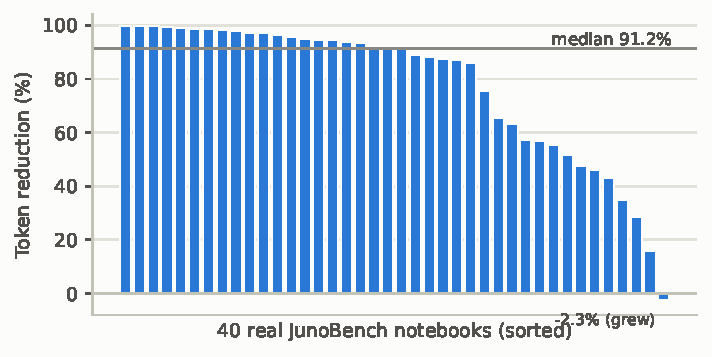
\includegraphics[width=.85\linewidth]{fig2_token_reduction.pdf}
\caption{Preprocessing shrinks real notebooks by a median of 91.2\%, with
a single, well-understood exception. Per-notebook token reduction on 40
real JunoBench notebooks, sorted. The single negative case is an
already-lean notebook that grows under YAML plus the state table.}
\label{fig:tokens}
\end{figure}

\subsection{Fair Notebook-NIAH: retrieval is not the failure mode; state is}
\label{sec:niah}
Notebook-NIAH is our adaptation of the ``needle in a haystack'' testing
idea used elsewhere to probe long-context recall: we hide a single target
value somewhere inside a long, synthetically generated notebook, and ask
the model to report it back. We swept three depths (0.1, 0.5, and 0.9 of
the way through the file) crossed with four lengths (roughly 8,000,
30,000, 60,000, and 100,000 tokens), all kept under a 126,000-token cap,
with three trials per grid cell (one trial per cell for the two 2026-03
model snapshots). In the \textbf{static} setting, the needle is placed
once and never reassigned; here gpt-4o scored 100\% for every condition
at every combination of depth and length, which tells us that noise
alone does not impair retrieval once a prompt actually fits in context,
correcting a claim we had assumed was true when we first started this
project. The \textbf{stateful} setting is the one that actually matters
for this paper's argument: here, the needle's true final value has the
highest \texttt{execution\_count} but appears \emph{earlier} in the
notebook's visual layout, while a decoy value sits later in the visual
order with a lower \texttt{execution\_count}, exactly mimicking the
real-world hazard described in Sect.~\ref{sec:causes}. We tested fifteen
models across seven vendors on this stateful setting: the nine OpenAI
models ran the full 36-trial grid, and six non-OpenAI models
(NVIDIA Nemotron-3-Super-120B, MiniMax-M3, Cohere North-Mini-Code,
InclusionAI Ling-3.0-Flash-Fin, Poolside Laguna-S-2.1, and Zhipu
GLM-5.3-Flash) ran a reduced grid of one length by three depths by one
or two trials by three conditions, sized to fit within each provider's
free-tier rate limit. The results appear in Figure~\ref{fig:curve}:
unaided (\texttt{raw}) accuracy ranges from 0\% for MiniMax-M3 and Cohere
North-Mini-Code up to 97\% for gpt-5 on the full grid. GLM-5.3-Flash
scored 100\% on its much smaller sample of only three trials, which is
too little evidence to treat as a reliable ceiling rather than a lucky
run. The compression-only control, \texttt{plain\_strip}, stayed close to
0\% throughout. Our full pipeline, \texttt{ours}, scored 100\% on every
single model. The component ablations on gpt-4o make the mechanism
clear: reordering alone (\texttt{reorder\_only}) also reaches 100\%,
while the state table alone with no reordering (\texttt{table\_only})
scores 0\%, the same as \texttt{plain\_strip}.

We draw five conclusions from this curve. First, reassigning a value out
of order degrades every model tested, even though the metadata needed to
resolve it correctly is sitting right there in the JSON; the failures
concentrate at the deepest positions in the file. Second, moving from
gpt-4o-mini to gpt-5 (a span of three OpenAI generations) took unaided
accuracy from 3\% to 97\%, but never closed the small remaining gap that
a deterministic serializer closes completely on every model at once,
using roughly 95\% fewer tokens in the process. In other words, model
scaling narrows the gap; it does not eliminate it the way reordering
does. Third, compression by itself does not help, and adding metadata
without also fixing the order does not help either: execution-order
reordering is both necessary and sufficient for this task on its own.
Fourth, accuracy does not increase smoothly with either model tier or
release date: gpt-4.1-nano actually outperforms the ostensibly stronger
gpt-4.1-mini, and the newer 2026-03 gpt-5.4-mini snapshot scores below
the earlier gpt-5-mini, so relying on serialization is a more predictable
lever than simply picking a newer model. Fifth, five of the six
non-OpenAI models reproduce the same pattern seen across the nine OpenAI
models: MiniMax-M3's 0\% raw score is the single worst result in the
entire curve, Nemotron-3-Super's 50\% sits in the middle of the pack, and
all six non-OpenAI models are fixed completely by \texttt{ours} once it
is applied. Because each non-OpenAI model only received three to six
trials on a reduced grid, we treat this as a spot check and not a
demonstration of broad cross-vendor generality: it tells us that five of
the six additional vendors did not contradict the main pattern, and that
the sixth (GLM-5.3-Flash) is too thinly sampled to draw any conclusion
from either way. We should also be transparent about a limitation of the
benchmark itself: because it is built to instantiate exactly the defect
JupPreprocessor is designed to fix, a perfect \texttt{ours} score mainly
confirms that the transform behaves correctly for that specific defect,
not that models generally prefer our output format in every setting. The
evidence we treat as load-bearing is the shape of the raw capability
curve together with the ablations, not the \texttt{ours}~=~100\% figure
taken on its own.

\begin{figure}[t]
\centering
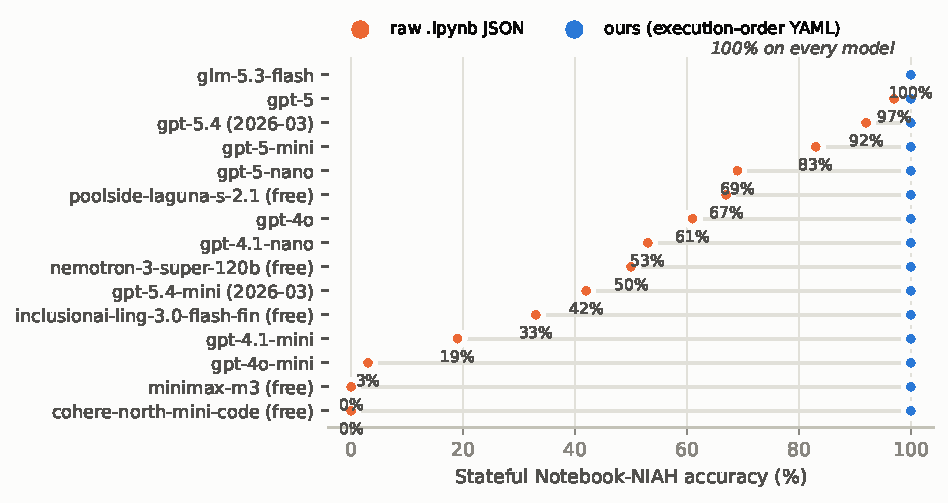
\includegraphics[width=.9\linewidth]{fig1_model_curve.pdf}
\caption{Execution-order reordering closes the state-tracking gap
completely on every model, while unaided accuracy varies enormously and
non-monotonically with model choice. Stateful Notebook-NIAH accuracy
across fifteen models: nine OpenAI models spanning four generations, plus
six non-OpenAI models (NVIDIA Nemotron-3-Super-120B, MiniMax-M3, Cohere
North-Mini-Code, InclusionAI Ling-3.0-Flash-Fin, Poolside Laguna-S-2.1,
Zhipu GLM-5.3-Flash) on a reduced grid, each via its own free tier.
Unaided (\texttt{raw}) accuracy spans 0\% to 97\% on every
adequately-sampled (full-grid) model and never reaches the 100\% that
execution-order reconstruction (\texttt{ours}) achieves on every model;
one thinly-sampled exception (GLM-5.3-Flash, $n=3$) also scored 100\%
raw, too small a sample to draw a conclusion from. \texttt{plain\_strip}
(not shown) is ${\approx}0\%$ throughout.}
\label{fig:curve}
\end{figure}

Table~\ref{tab:modelcurve} gives the exact per-model numbers underlying
Figure~\ref{fig:curve}, since a figure alone can be hard to read precisely
for fifteen separate models.

\begin{table}[t]
\centering\small
\begin{tabular}{@{}lccc@{}}
\toprule
Model & \texttt{raw} & \texttt{plain\_strip} & \texttt{ours} \\
\midrule
gpt-4o & 61\% (22/36) & 0\% (0/36) & 100\% (36/36) \\
cohere-north-mini-code (free) & 0\% (0/3) & 0\% (0/3) & 100\% (3/3) \\
glm-5.3-flash & 100\% (3/3) & 33\% (1/3) & 100\% (3/3) \\
gpt-4.1-mini & 19\% (7/36) & 0\% (0/36) & 100\% (36/36) \\
gpt-4.1-nano & 53\% (19/36) & 8\% (3/36) & 100\% (36/36) \\
gpt-4o-mini & 3\% (1/36) & 0\% (0/36) & 100\% (36/36) \\
gpt-5 & 97\% (35/36) & 8\% (3/36) & 100\% (36/36) \\
gpt-5-mini & 83\% (30/36) & 0\% (0/36) & 100\% (36/36) \\
gpt-5-nano & 69\% (25/36) & 0\% (0/36) & 100\% (36/36) \\
gpt-5.4 (2026-03-05) & 92\% (11/12) & 0\% (0/12) & 100\% (12/12) \\
gpt-5.4-mini (2026-03-17) & 42\% (5/12) & 0\% (0/12) & 100\% (12/12) \\
inclusionai-ling-3.0-flash-fin (free) & 33\% (1/3) & 0\% (0/3) & 100\% (3/3) \\
minimax-m3 (free) & 0\% (0/6) & 0\% (0/6) & 100\% (6/6) \\
nemotron-3-super-120b (free) & 50\% (3/6) & 0\% (0/6) & 100\% (6/6) \\
poolside-laguna-s-2.1 (free) & 67\% (2/3) & 0\% (0/3) & 100\% (3/3) \\
\bottomrule
\end{tabular}
\caption{Exact per-model accuracy on the stateful Notebook-NIAH benchmark.
The nine OpenAI models ran the full 36-trial grid; the six non-OpenAI
models ran a reduced grid (3--6 trials) sized to each provider's free-tier
rate limit. \texttt{ours} is 100\% on all fifteen models with no
exception. Compiled automatically from per-model reports; see
\texttt{reports/model\_curve\_report.md}.}
\label{tab:modelcurve}
\end{table}

\subsection{State hazards are the norm in the debugging population}
\label{sec:scan}
We scanned all 112 original JunoBench notebooks for the two static
warning signs a preprocessor can actually detect without executing
anything: a mismatch between visual and execution order, and gaps in the
\texttt{execution\_count} sequence that indicate a cell was re-run or
deleted. We found that 59.8\% of these notebooks are non-monotonic
(their visual order does not match their execution order), 89.3\% show
execution-count gaps (a precondition for the ghost-variable problem
described in Sect.~\ref{sec:causes}), and 92.0\% show at least one of
these two hazards. Compared with the roughly 36\% figure reported for
GitHub notebooks in general \citep{siddik2025}, this suggests that the
specific notebooks most likely to be handed to an LLM for help are also
the ones most likely to mislead it.

\subsection{Executable ground truth on real notebooks}
\label{sec:realnb}
To find out whether real notebooks actually contain the kind of
order-divergent variable our synthetic benchmark is built to test, we
took every out-of-order notebook we could identify and executed it twice
inside an isolated sandbox, once sorted by \texttt{execution\_count} and
once in its original visual order, using identical random seeds and
per-cell timeouts for both runs. We first installed
\texttt{torch}/\texttt{torchvision} (CPU wheels, Python 3.14), and later
widened the corpus further using a separate Python 3.12 virtual
environment with TensorFlow, since no TensorFlow wheel exists for Python
3.14 at the time of writing. This let 62 of 67 candidate notebooks
execute usefully, yielding 52 order-divergent variables across 16
notebooks. This is a conservative lower bound: several notebooks still
could not fully execute because of missing data files or heavy
dependencies, one TensorFlow notebook remains unexecutable because a
large mid-execution network download races against our per-cell timeout
(a genuine flaky-network issue rather than a missing-dependency one), and
we observed run-to-run variance of 52 to 55 items across repeated
extraction runs, traced to other network-dependent code inside the
notebooks themselves. We found two distinct kinds of divergence. The
first is \emph{value divergence}: in \texttt{sklearn\_9}, the model that
actually exists at the end of the session is a plain
\texttt{LogisticRegression()}, while a naive visual-order reading would
conclude it is
\texttt{LogisticRegression(solver='liblinear')}. The second is
\emph{existence divergence}, which introduces what we call
\textbf{phantom variables}: the mirror image of a ghost variable, in that
the code defining it is visible in the file but the definition itself
never actually completed successfully during the real session.
Table~\ref{tab:realnb} breaks the 52 items down by notebook and
divergence type: the distribution is uneven by design rather than by
selection, since some notebooks simply contain far more order-divergent
variables than others once actually executed.

\begin{table}[t]
\centering\small
\begin{tabular}{@{}lccc@{}}
\toprule
Notebook & Items & Value divergence & Existence divergence \\
\midrule
\texttt{NBspecific\_10.ipynb} & 1 & 0 & 1 \\
\texttt{NBspecific\_11.ipynb} & 2 & 0 & 2 \\
\texttt{NBspecific\_15.ipynb} & 1 & 1 & 0 \\
\texttt{matplotlib\_1.ipynb} & 4 & 4 & 0 \\
\texttt{numpy\_1.ipynb} & 12 & 0 & 12 \\
\texttt{numpy\_11.ipynb} & 8 & 1 & 7 \\
\texttt{pandas\_3.ipynb} & 5 & 0 & 5 \\
\texttt{sklearn\_7.ipynb} & 1 & 0 & 1 \\
\texttt{sklearn\_9.ipynb} & 3 & 1 & 2 \\
\texttt{torch\_10.ipynb} & 1 & 1 & 0 \\
\texttt{torch\_11.ipynb} & 1 & 1 & 0 \\
\texttt{torch\_3.ipynb} & 6 & 1 & 5 \\
\texttt{torch\_4.ipynb} & 1 & 0 & 1 \\
\texttt{torch\_6.ipynb} & 3 & 0 & 3 \\
\texttt{torch\_7.ipynb} & 1 & 1 & 0 \\
\texttt{torch\_8.ipynb} & 2 & 0 & 2 \\
\midrule
Total (16 notebooks) & 52 & 11 & 41 \\
\bottomrule
\end{tabular}
\caption{The 52 real order-divergent variables by notebook and
divergence type. Existence divergence (phantom variables) accounts for
the large majority (41 of 52); value divergence, where a variable exists
under both readings but holds a different value, accounts for the
remaining 11. \texttt{numpy\_1.ipynb} alone contributes 12 items, all
existence divergence, and is the notebook responsible for the
\texttt{execution\_count}-sort edge case discussed in
Sect.~\ref{sec:threats}.}
\label{tab:realnb}
\end{table}

We then asked gpt-4o to report the final state of each of the 52 items
under three serializations, and graded its answers with a three-way
judge: \textsc{truth} means the answer matches the execution-order state,
\textsc{decoy} means it matches the (wrong) visual-order state, and
\textsc{neither} means it matches neither stored candidate. The results,
after fixing a judge bug we describe below, appear in
Figure~\ref{fig:realstate}, together with 95\% Wilson confidence
intervals (a standard way of expressing our uncertainty about a
proportion measured from a limited number of trials) on the
overall-truth rate: raw 23\% [14, 36], \texttt{plain\_strip} 27\% [17,
40], \texttt{ours} 27\% [17, 40]. We report four findings here, arrived
at only after three separate rounds of self-correction. The first and
most robust finding, unchanged by any of those corrections and if
anything strengthened by them, concerns simple \textbf{access}: the raw
JSON file is too large to fit in context for 62\% of these real
divergent items at $n=52$, up from 51\% at an earlier $n=41$ snapshot,
since larger real notebooks kept entering the corpus as we widened it;
our serializer reaches 85\% of items and \texttt{plain\_strip} reaches
83\%. The second finding is less flattering: once an answer is actually
given, we find \emph{no} distinguishable accuracy advantage for
\texttt{ours}. It is tied with \texttt{plain\_strip} at 27\% overall
truth, raw trails only nominally at 23\%, and all three confidence
intervals overlap heavily. This matches the conclusion we already reached
at $n=41$ after fixing the judge bug, so the larger sample confirmed the
finding instead of reversing it.

The third finding is about the correction process itself, and we
consider it worth reporting as a finding in its own right, broken here
into its four separate stages.

\textbf{Initial pilot.} An initial 13-item pilot looked like a clean win
for our method, at 6 out of 13 correct versus raw's 3 out of 13.
Expanding to 41 items narrowed this gap to something indistinguishable
from noise.

\textbf{Judge bug and bias.} A manual audit of the automated gpt-4o-mini
judge, in which we independently re-checked 25 of 123 answer rows by
hand (Sect.~\ref{sec:judgeaudit}), then uncovered a 24\% disagreement
rate concentrated in a single, specific mechanism: whenever one of the
two stored ground-truth candidates was ``the variable was never
defined,'' the judge tended to credit any other concrete-looking answer
to the remaining candidate without actually checking whether the value
matched. This bug happened to favor our method's tendency to produce a
confident, specific-looking guess from its variable table, even when
that guess was wrong.

\textbf{Post-fix result.} Once we rewrote the judge's prompt to require
an explicit literal or close value match, our method's apparent
advantage disappeared entirely.

\textbf{Expanded corpus confirmation.} Expanding the corpus a second
time, to 52 items via the newly built TensorFlow environment, reproduced
this corrected, more modest result instead of reversing it again. We
report all four stages of this progression, not only the final number,
because each successive correction moved the conclusion in the same
direction: toward a more modest and, we believe, more trustworthy claim.

\subsection{Judge validation}
\label{sec:judgeaudit}
To check the automated judge's reliability directly, a member of our
project team manually re-graded 25 of 123 answer rows by comparing each
sampled answer against the stored ground-truth candidates by hand,
without invoking any LLM classifier in that re-check. The 25 rows were a
stratified random sample (seed 42), not a sample selected after looking
for suspected problem cases: we fixed the random seed before drawing the
sample, so the audit could not have been enriched with rows we already
suspected were wrong. This produced 19
out of 25 (76\%) agreement with the original automated judge. All six
disagreements shared one underlying cause, which we can demonstrate with
a single reproducible example: for \texttt{numpy\_1.ipynb}'s
\texttt{device} variable, where the truth candidate was ``never defined''
and the decoy candidate was the literal string \texttt{cpu}, the
identical answer text \texttt{cuda} was graded \textsc{decoy} under one
serialization condition and \textsc{truth} under another. Neither grade
was actually correct, since \texttt{cuda} matches neither stored
candidate. We rewrote the judge's prompt to require an explicit literal
or close value match, and to default to \textsc{neither} whenever this
is uncertain. We also began persisting the model's full, untruncated
answers for future audits
(\texttt{tests/real\_state\_eval\_raw\_answers.json}). Full detail is
available in \texttt{reports/judge\_validation\_report.md}.

\textbf{Post-fix confirmation.} A prompt fix is only as trustworthy as the
next independent check of it, so we repeated this audit on a second,
non-overlapping sample after applying the fix: 25 further rows, stratified
by condition, drawn with a different random seed (7) from the corrected-judge
dataset. Agreement rose from 76\% to 92\% (23 of 25). The two remaining
disagreements were both the same underlying variable
(\texttt{pandas\_3.ipynb}'s \texttt{resultados}), where the judge credited a
fully-populated DataFrame answer as matching a stored decoy candidate that is
literally an \emph{empty} DataFrame with matching column names but no rows,
a narrower, DataFrame-specific failure mode distinct from the null-candidate
bug described above. We report this as a residual limitation rather than a
clean bill of health: readers should continue to treat the exact
\textsc{truth}/\textsc{decoy}/\textsc{neither} counts in
Sect.~\ref{sec:realnb} as approximate, with the qualitative conclusion, no
detectable accuracy advantage at this scale, being what we actually stand
behind rather than any single precise tally. Full detail is in
\texttt{reports/judge\_post\_fix\_validation\_report.md}.

\begin{figure}[t]
\centering
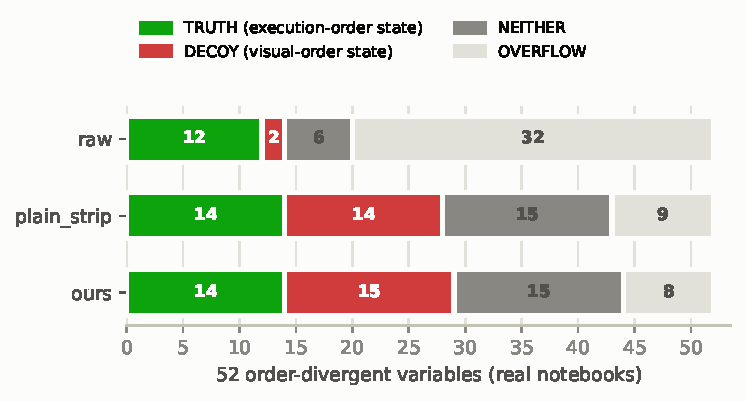
\includegraphics[width=.85\linewidth]{fig3_real_state_outcomes.pdf}
\caption{Raw JSON's biggest problem on real notebooks is fitting in
context at all, not accuracy once it does: \textsc{overflow} dominates
its outcome bar, while \texttt{ours} and \texttt{plain\_strip} reach far
more items without a matching gain in \textsc{truth}. Outcomes on the 52
real order-divergent variables per serialization. \textsc{overflow} = the
prompt could not fit the 126k context cap.}
\label{fig:realstate}
\end{figure}

\subsection{Honest negatives}
\label{sec:honestneg}
On the Themisto benchmark \citep{grotov2025themisto}, whose notebooks
were already cleaned of HTML, base64 content, and JSON metadata by its
own authors, applying our preprocessing actually \emph{reduced}
output-prediction accuracy, from 40.0\% down to 26.7\%, while also adding
token overhead rather than removing it. We did not simply accept the
published explanation for this at face value; instead, we measured the
actual breakdown of where the errors occurred, and found the original
explanation was wrong. Of the items our method answered incorrectly, most
(9 of 11) were \emph{also} answered incorrectly under the raw condition,
because both formats were guessing at data that neither one actually had
access to; only 2 of the 15 items in this sample decided the entire gap
between the two conditions. In both of those two decisive items, the
correct value was present verbatim in our preprocessed prompt; it had not
been stripped or lost anywhere. What we found instead, by measuring
character distances directly, is that the variable-state table our
pipeline inserts between the notebook's code history and the final query
pushes the correct evidence 2.7 to 7.7 times farther from the point where
the model must answer than it sits in the raw format, and in both cases
the model's wrong answer matched a closer but incorrect value shown
elsewhere in the same prompt. This looks like a lost-in-the-middle effect,
where information further from the point of decision is used less
reliably, and not an information-loss effect where the value was simply
missing. Structure is a net negative specifically in a setting like this
one, where there was no token bloat to strip in the first place, so
adding structure only adds distance without buying back any savings.
Separately, on a full-context JunoBench debugging check, accuracy was
identical (8 of 8 correct under both conditions) while our version used
79.1\% fewer tokens: a cost result, not an accuracy result.

We want to state plainly what this Themisto result does and does not
mean for the method as a whole. It does not mean the method generally
hurts accuracy: on Themisto specifically, there was no token bloat to
remove in the first place, so the only thing our added structure could
do was push evidence farther from the query, which is exactly what
happened. Our method's actual strength lies in bloated, scrambled
notebooks like the JunoBench corpus used throughout this paper, not in
notebooks that are already lean and already in the correct order. A
practitioner deciding whether to apply JupPreprocessor to a given
notebook should weigh how bloated and how out-of-order it actually is,
not assume the tool is a uniform improvement regardless of input.

\section{Threats to Validity}
\label{sec:threats}

\subsection{Construct validity}
The Notebook-NIAH synthetic benchmark is, by its own construction,
favorable to our method: it deliberately instantiates the exact defect
(a value reassigned out of order) that JupPreprocessor is designed to fix,
so a perfect score on \texttt{ours} mainly confirms that the transform is
correct and complete for that specific defect. It does not by itself show
that language models generally prefer our output format in other
settings. To be explicit about the boundary of this claim: Notebook-NIAH
tests exactly one of the six state hazards named in Sect.~\ref{sec:causes},
non-linear execution (cause A). It does not instantiate in-place
mutation (B), ghost variables (C), re-execution divergence (D), silenced
errors (E), or environment-dependent branching, and we do not claim that
``execution-order reconstruction is necessary and sufficient'' extends to
any of those other hazards; it is a claim about this one benchmark's one
failure mode, not about notebook state tracking in general. We treat the benchmark's controls
(\texttt{plain\_strip}, \texttt{reorder\_only}, \texttt{table\_only})
together with the independent real-notebook study as the evidence that
actually matters here, not the \texttt{ours}~=~100\% figure taken in
isolation.

The automated LLM judge used for real-notebook grading (gpt-4o-mini) had
a measured 24\% disagreement rate with independent manual re-grading
before we found and fixed the bug behind it (Sect.~\ref{sec:judgeaudit});
readers should treat the exact TRUTH and DECOY counts as approximate
even after the fix, since no fully human-annotated ground truth exists
for this task.

\texttt{execution\_count}-sort
itself also has a real, verified construct-validity problem of its own:
this field only records a cell's \emph{most recent} run, not a
mutually-consistent history of the whole session, so an early cell that
gets re-run late (for example, an import statement re-executed after a
kernel restart) can end up sorted \emph{after} code that already depends
on it. The resulting order is not something you could actually replay in
a fresh kernel, and it does not correspond to any real moment in the
notebook's history. We verified this directly in \texttt{numpy\_1.ipynb},
where an import cell carries $\texttt{execution\_count}{=}27$ while a
cell that needs \texttt{torch} carries $\texttt{execution\_count}{=}2$
(see \texttt{reports/execution\_count\_reordering\_limitation.md}); our
new \texttt{execution\_order\_risk} annotation correctly fires on exactly
the 6 cells affected by this issue. An earlier, smaller snapshot of the
ground-truth corpus ($n{=}41$, before we expanded it to $n{=}52$ using
the Python 3.12 and TensorFlow environment) estimated that this mechanism
plausibly explained 8 of those 41 items, 7 from \texttt{numpy\_1.ipynb}
and 1 from \texttt{torch\_4.ipynb}, rather than genuine
out-of-order-execution divergence. We have not re-quantified this
specific estimate at $n{=}52$, so we flag it here as an estimate carried
over from an earlier snapshot of the corpus rather than a current,
re-verified count. Both our tool and the ground-truth methodology inherit
this same underlying assumption regardless. A separate, corpus-wide
static scan that cost nothing and made no LLM calls
(\texttt{reports/execution\_count\_consistency\_report.md}), restricted
to names bound by an \texttt{import} statement for a cleaner signal than
a noisier count dominated by ordinary reuse of short generic variable
names, found that this issue affects \textbf{29 of 109 analyzable
JunoBench notebooks (26.6\%)}, which is common enough to be worth fixing
directly. The preprocessor now does exactly that: a new
\texttt{execution\_order\_risk} per-cell annotation, verified against the
6 affected cells in \texttt{numpy\_1.ipynb}, passes the full existing
unit test suite, and costs a negligible amount of extra tokens. We chose
this detect-and-flag approach over a more ambitious hybrid reordering fix
because it is the lower-risk option, and because it is consistent with
this paper's own three-tier philosophy of flagging uncertainty honestly
instead of guessing at an answer we cannot actually verify.

\textbf{A related, tested-but-inconclusive hypothesis.} We also tested a related hypothesis directly instead of leaving it as
an untested guess: that environment-dependent branching, meaning checks
such as \texttt{torch.cuda\allowbreak.is\_available\allowbreak()} whose
outcome depends on the machine the code happens to run on rather than
anything visible in the file itself, might be a separate static-analysis
blind spot distinct from the \texttt{execution\_count}-sort issue
described above. The result of this test was genuinely inconclusive, and
we report it as such. 8 of the 41 items in our earlier ground-truth
snapshot matched an environment-branching pattern, and the raw
correlation looked striking at first glance: an 88.2\% wrong-answer rate
for these flagged items, compared with 48.1\% for items without the flag.
However, every one of those 8 flagged items shares the identical
\texttt{phantom\_in\_visual}/\texttt{ec\_order\_value=None} signature
already fully explained by the \texttt{execution\_count}-sort mechanism
above, so this particular corpus contains zero cases that could actually
separate the two hypotheses from each other. We report this honestly as
an inconclusive result: it is not evidence that the environment-branching
hypothesis is false, only evidence that this specific corpus happens to
be unable to test it one way or the other. We think a tested-but-inconclusive
hypothesis is still worth keeping in the record instead of quietly
dropping it.
(\texttt{reports/environment\_branching\allowbreak\_check.md})

\subsection{Internal validity}
At $n{=}52$, after fixing the judge bug identified above and replicating
the result across $13\to41\to52$ items, \texttt{ours} shows no
accuracy-when-answered advantage over \texttt{raw} or over the plain
compression control (\texttt{plain\_strip}): \texttt{ours} and
\texttt{plain\_strip} are tied at 27\%, and \texttt{raw} trails only
nominally at 23\%, all within noise. Because the same 52 items are
scored under all three conditions, we also report a paired risk
difference rather than only comparing separate confidence intervals:
\texttt{ours} beats \texttt{raw} on 6 items and loses to it on 4, for a
paired risk difference of $+3.8$ percentage points (95\% CI
$[-8.0, +15.7]$); \texttt{ours} beats \texttt{plain\_strip} on 3 items and
loses to it on 3, for a paired risk difference of exactly $0.0$ percentage
points (95\% CI $[-9.2, +9.2]$). Both intervals contain zero by a wide
margin, which is a more direct way of saying the same thing as the
overlapping Wilson intervals above: at this sample size, we cannot
distinguish \texttt{ours} from either baseline on a per-item basis. The
real-notebook claim this paper
actually stands behind rests entirely on reach and coverage, not on any
demonstrated per-item accuracy advantage of structure over compression.
This is a further downgrade from an already-downgraded 13-item and then
41-item pre-fix draft, and we report it transparently as such: this
result got smaller and more modest at every stage we checked it, not
larger. We did not carry out a formal power analysis before concluding
that this is a genuine null result rather than simply an underpowered
one; at the effect sizes we actually observed, a substantially larger
item count, plausibly 150 or more, would be needed to resolve the
question with real confidence, and we flag this explicitly as an open
question instead of treating our current $n{=}52$ as the final word.
Real-notebook state accuracy in this paper is therefore a 52-item case
study covering the full population we could recover across a Python 3.14
environment with torch and torchvision, plus a separate Python 3.12
environment with TensorFlow, not a random sample of notebooks in general.
One TensorFlow notebook remains unexecutable because of a flaky,
timeout-sensitive network download rather than a missing dependency, and
we observed run-to-run item-count variance of 52 to 55 due to genuinely
network-dependent code inside the notebooks themselves. Finally, static
extraction cannot detect the runtime failure of code that looks
syntactically valid; these phantom-variable cases are, in fact, the
dominant remaining source of error regardless of which serialization
condition is used.

\subsection{External validity}
Fifteen answer models in total were tested on the synthetic stateful
benchmark: nine are from OpenAI, and six (NVIDIA Nemotron-3-Super-120B,
MiniMax-M3, Cohere North-Mini-Code, InclusionAI Ling-3.0-Flash-Fin,
Poolside Laguna-S-2.1, and Zhipu GLM-5.3-Flash, each accessed through its
own provider's free tier) are not. The non-OpenAI models ran a reduced
grid of one length by three depths by one or two trials by three
conditions, sized to fit inside each provider's rate limit.
\texttt{ours} scores 100\% on all six of these models regardless; five of
the six reproduce the qualitative pattern of imperfect, non-monotonic
\texttt{raw} accuracy seen throughout the OpenAI curve, while the sixth
(GLM-5.3-Flash) scored 100\% raw on only three trials. We consider this
reassuring, but three to six trials per non-OpenAI model on a reduced
grid is not enough to claim broad cross-vendor generality on its own; it
tells us that most of these six additional vendors did not contradict the
pattern, not that we have demonstrated general cross-vendor
independence, and the one exception is too thinly sampled to interpret
in either direction. Two further free-tier candidates, Google Gemma-4-31B
and NVIDIA Nemotron-3-Ultra-550B, along with a Gemini 3.7/3.8 Flash
attempt, were tried and then dropped after we confirmed persistent
upstream unavailability: exhausted retries in the first two cases, and
repeated HTTP 400 and 503 errors traced specifically to free-tier
capacity limits (not to our own account, since we confirmed this was
reproducible with two independent API keys) in the Gemini case. This
follows our project's standing policy of dropping a source that has
proven consistently unreliable rather than continuing to fight it or
reporting a data point we cannot trust. The real-notebook evaluation used
gpt-4o exclusively. All of our real-notebook data comes from a single
benchmark corpus, JunoBench, so we have not tested how well our findings
generalize to notebooks outside this specific crashed-machine-learning
population. On the cost of Tier 3, our runtime-verification tier
(Sect.~\ref{sec:causes}): we already restrict this tier's use to settings
where a live kernel is genuinely available, and the outside evidence we
found supports keeping that restriction and does not suggest it is
overly cautious. A 2026 preprint (FlowBook) reports lightweight dynamic
instrumentation with a median overhead of 70 milliseconds per cell,
which is cheap, but only while a notebook is \emph{already executing}.
That is not a way to validate one isolated cell in the absence of a
kernel, so it does not relax our own no-kernel constraint for Stage 1; it
only suggests that Tier 3 is less costly than we might otherwise assume
in settings, such as an interactive agent session, where a kernel is
already attached for some other reason.

\section{Related Work}
\label{sec:relwork}
Several notebook agents and stateful runtimes, including DatawiseAgent
\citep{you2025datawise}, CaveAgent \citep{ran2026caveagent}, DeltaBox
\citep{dong2026deltabox}, and I-PTC \citep{gonzalez2026}, all assume a
live kernel is available. Serialization-side tooling that does not
assume a kernel tends to be lossy: Jupytext \citep{jupytext} and
notebookllm \citep{notebookllm} both strip outputs entirely, and existing
base64-stripping tools have not, to our knowledge, been formally
evaluated for their effect on model accuracy. Existing benchmarks,
including Themisto \citep{grotov2025themisto}, JunoBench
\citep{wang2025junobench}, NbQA/Jupiter \citep{li2025jupiter}, and
DABStep \citep{egg2025dabstep}, test downstream tasks rather than
serialization formats themselves; none of them isolate execution-order
reconstruction as an independent variable the way we do here. As far as
we are aware, no prior work measures LLM state accuracy against
dual-order executable ground truth on real notebooks. Table~\ref{tab:relwork}
summarizes, for the four prior systems discussed in detail below, what
each one actually measures and how that differs from our own evaluation.

\begin{table}[t]
\centering\small
\begin{tabular}{@{}p{2.4cm}p{2.5cm}p{2.0cm}p{2.0cm}p{3.1cm}@{}}
\toprule
System & Task & Live kernel? & Serialization a variable? & Headline result \\
\midrule
CRABS \citep{li2025crabs} & Execution-dependency graph reconstruction & No; LLM disambiguation step instead & No; fixed input format & 98--99\% F1 on 50 curated Kaggle notebooks \\
LongDS-Bench \citep{xu2026longds} & Long-horizon analytical state maintenance & Yes; agent executes tools & No & Best model 48.45\% accuracy; $\sim$47-pt drop late in session \\
DSAgentBench \citep{rahman2026dsagentbench} & End-to-end data-science workflow completion & Yes; real computer environment & No & Best model 56.70\% task success \\
marimo \citep{marimo} & Reactive execution, no serialization step & Yes, by design & N/A; format itself is the fix & 40/40 tooling-reliable, 40/40 blocked by missing deps/data (this paper's test) \\
\textbf{This paper} & State-tracking under a controlled serialization change & No; static, zero-LLM-cost & Yes; the independent variable & 100\% synthetic, null real-notebook accuracy, coverage gain confirmed \\
\bottomrule
\end{tabular}
\caption{How the closest prior systems compare to this paper along the
dimensions that matter for our claim. None of the four vary serialization
format as a controlled experimental variable the way we do; three of the
four require a live kernel or agent-executed environment that our
zero-LLM-cost, no-kernel setting is specifically designed to avoid
needing.}
\label{tab:relwork}
\end{table}

The closest prior work to ours is \textbf{CRABS} \citep{li2025crabs}
(COLM 2025), which reconstructs a notebook's execution-dependency graph
using static and syntactic analysis combined with an LLM disambiguation
step, reporting 98--99\% F1 on 50 real Kaggle notebooks. This is
meaningful evidence that a static-analysis-plus-LLM approach can recover
a notebook's execution structure without actually re-executing it.
CRABS's accuracy, however, depends on that LLM step, which places it
closer to our optional Stage 2 than to our zero-LLM-cost Stage 1 taken on
its own; its evaluation sample of ``highly-upvoted'' Kaggle notebooks is
also noticeably cleaner than the crashed, messy corpus we study here, so
we do not know whether CRABS's accuracy would transfer to a harder
setting like ours. Two more recent benchmarks independently support the
broader motivation for this work, beyond the older reproducibility
literature we already cite: \textbf{LongDS-Bench} \citep{xu2026longds}
finds that even the best model reaches only 48.45\% accuracy at
maintaining and restoring analytical state across long-horizon tasks
derived from real Kaggle notebooks, with a roughly 47-point accuracy drop
from early to late turns that the authors attribute to a genuine failure
to maintain state rather than simply running out of interaction budget;
and \textbf{DSAgentBench} \citep{rahman2026dsagentbench} finds that the
best model succeeds on only 56.70\% of 275 real, full-environment
data-science tasks. Neither benchmark targets serialization directly, but
both reinforce our motivating claim that state-tracking during
notebook-style analysis remains an unsolved problem at the level of
whole agent systems, not simply a niche concern within the older
reproducibility literature.

A structurally different alternative to our approach is
\textbf{reactive, or dataflow, notebooks such as marimo}
\citep{marimo}, which eliminate hidden state and out-of-order execution
by design instead of by reconstructing it after the fact, at the cost
of requiring a conversion away from the standard \texttt{.ipynb} format.
We tested marimo's own official conversion tooling
(\texttt{marimo convert} followed by \texttt{marimo export html}) on the
same 40-notebook real, crashed corpus used in Sect.~5.1. Conversion and
reactive execution never crashed or timed out on any of the forty
notebooks, but every single one of them had at least one cell fail
during execution, almost always because of missing local data files or
third-party packages not present in the runtime environment, which is
the same ``missing dependency or data'' failure mode our own dual-order
re-execution ground truth already reports for these same notebooks. We
read this as evidence \emph{in favor of}, not against, a static,
execution-free approach on the specific question of reach: any method
that requires live execution, marimo's reactive model included, inherits
the same real-world unavailability of a notebook's original data and
environment, while a purely static method cannot be blocked by a missing
file or package because it never attempts to run anything at all. We did
not compare marimo's own recovered variable states against our
executable ground truth in the cases where both approaches actually can
execute successfully; that comparison remains open for future work. We
emphasize that this experiment tested only reach and executability, not
comparative state accuracy, and it should be read with that scope in
mind rather than as a claim that our static approach is more accurate
than marimo's reactive one.
(\texttt{reports/marimo\_conversion\_report.md})

\section{Conclusion}
This paper is built around two defects and one underlying mechanism:
strip what the file wastes, reconstruct what it scrambles, and be
explicit about what cannot actually be known. In a fair, controlled
synthetic setting, execution-order reconstruction is both necessary and
sufficient to fix the measurable state-tracking failure we identified, at
roughly 95\% fewer tokens and effectively no added inference-time cost.
That result does not, however, transfer cleanly to real notebooks as an
accuracy advantage. On 52 real order-divergent variables from 16
crashed machine-learning notebooks, using gpt-4o as the sole answer
model, our serializer and a plain compression control are statistically
tied, and the raw file trails both, all within noise once an answer is
actually reached, and this conclusion held when we expanded the corpus
from 41 to 52 items rather than reversing itself. We want to be precise
about what this null result does and does not license: it is evidence
against an accuracy advantage for gpt-4o on this specific, deliberately
hard population of crashed ML notebooks, not a general claim about every
model or every kind of notebook. Whether the same null result holds for
other answer models, or for calmer notebook populations such as teaching
or exploratory data analysis, remains untested and is the most direct
follow-up this paper's own evidence calls for. What does transfer, and what we are
prepared to stand behind, is narrower but still substantial: raw JSON is
frequently unusable on real notebooks at all, overflowing context on 62\%
of real divergent items, and this gap widened instead of narrowing as we added
more real notebooks to the corpus, while a deterministic, zero-LLM-cost
serializer keeps the notebook readable almost every time. On real, messy
data, then, a serializer that is honest about what it does not know
functions first as a coverage tool, and only potentially later as an
accuracy tool. Even under close scrutiny of our own pipeline, including a
judge bug we found and fixed and an edge case in our own reordering
mechanism that we also found and fixed, this particular coverage claim
held up.

For someone building a notebook agent today, we would summarize the
practical guidance as follows. Deploy JupPreprocessor when notebooks are
bloated, out of order, or otherwise at risk of overflowing context,
since that is where the coverage gain is real and, on the evidence
gathered here, essentially free. Do not expect an accuracy improvement
on notebooks that are already lean and already in execution order; on
such notebooks, added structure can hurt rather than help, as the
Themisto result shows. Treat the \texttt{execution\_order\_risk} flag as
a signal to fall back to a more conservative, uncertainty-preserving
reading of the affected cells, not as confirmation that anything is
actually broken; it fires on a real but specific pattern (a cell re-run
late in a session) that neither our tool nor a live re-execution can
fully resolve without more information than the file itself contains.

\section*{Statements and Declarations}

\paragraph{Funding.} No external funding was received for this work.

\paragraph{Competing interests.} The author declares no competing financial
or non-financial interests directly or indirectly related to this work.

\paragraph{Author contributions.} Single-author manuscript: MD.\ Raiyan Bin
Rafique conceived the study, designed and ran all experiments (with the
LLM-assistance disclosed in Sect.~\ref{sec:llmuse}), analyzed the results, and
wrote the manuscript.

\paragraph{Ethical approval.} This study did not involve human participants,
animal subjects, or personally identifying data; no ethical approval was
required. All notebook data is drawn from JunoBench, a publicly released,
pre-existing benchmark of crashed machine-learning notebooks
\citep{wang2025junobench}.

\paragraph{Clinical trial number.} Not applicable.

\paragraph{Data availability.} The complete source code for
JupPreprocessor, the evaluation harnesses (Notebook-NIAH, the real-notebook
dual-order ground-truth extractor, the Themisto and JunoBench evaluation
scripts), all measured reports underlying every quantitative claim in this
manuscript, and the full project changelog documenting the correction
history described in Sect.~\ref{sec:realnb}--Sect.~\ref{sec:judgeaudit} are
available at
\url{https://github.com/hodini007/notebook-research}.
EMSE's editorial policy states that submissions missing required
declarations will be returned as incomplete.

\bibliographystyle{apalike}
\begin{thebibliography}{20}
\raggedright

\bibitem[Dong et al.(2026)Dong, He, Liu, Hou, Du, Xu, Yu, and Yang]{dong2026deltabox}
Dong Y, He J, Liu S, Hou Y, Du D, Xu Z, Yu S, Yang B (2026) DeltaBox: Scaling
Stateful AI Agents with Millisecond-Level Sandbox Checkpoint/Rollback.
arXiv:2605.22781. \url{https://arxiv.org/abs/2605.22781}

\bibitem[Egg et al.(2025)Egg, Iglesias Goyanes, Kingma, Mora, von Werra, and Wolf]{egg2025dabstep}
Egg A, Iglesias Goyanes M, Kingma F, Mora A, von Werra L, Wolf T (2025)
DABstep: Data Agent Benchmark for Multi-step Reasoning. arXiv:2506.23719.
\url{https://arxiv.org/abs/2506.23719}

\bibitem[Gonzalez(2026)]{gonzalez2026}
Gonzalez J (2026) Toward Stateful Execution Interfaces for Language Model
Agents. Technical Report UCB/EECS-2026-176, EECS Department, University of
California, Berkeley.
\url{https://www2.eecs.berkeley.edu/Pubs/TechRpts/2026/EECS-2026-176.html}

\bibitem[Grotov and Titov(2025)]{grotov2025themisto}
Grotov K, Titov S (2025) Themisto: Jupyter-Based Runtime Benchmark.
arXiv:2504.12365. Accepted to the Third Deep Learning for Code (DL4C)
Workshop @ ICLR 2025. \url{https://arxiv.org/abs/2504.12365}

\bibitem[Jupytext(2026)]{jupytext}
Jupytext (2026) Jupytext documentation and command-line reference.
\url{https://jupytext.readthedocs.io/en/latest/using-cli.html}. Accessed 6
September 2026.

\bibitem[Li et al.(2025a)Li, McPhillips, Wang, Tsai, and Ludäscher]{li2025crabs}
Li M, McPhillips TM, Wang D, Tsai SR, Ludäscher B (2025) CRABS: A
syntactic-semantic pincer strategy for bounding LLM interpretation of Python
notebooks. arXiv:2507.11742. Accepted to COLM 2025.
\url{https://arxiv.org/abs/2507.11742}

\bibitem[Li et al.(2025b)Li, Liu, Du, Zeng, Xu, Zhou, He, and Dong]{li2025jupiter}
Li S, Liu Y, Du S, Zeng W, Xu Z, Zhou M, He Y, Dong H (2025) Jupiter:
Enhancing LLM Data Analysis Capabilities via Notebook and Inference-Time
Value-Guided Search. arXiv:2509.09245. Accepted to AAAI 2026.
\url{https://arxiv.org/abs/2509.09245}

\bibitem[marimo(2026)]{marimo}
marimo (2026) marimo documentation: Reactivity.
\url{https://docs.marimo.io/guides/reactivity/}. Accessed 6 September 2026.

\bibitem[notebookllm(2026)]{notebookllm}
notebookllm (2026) notebookllm package, Python Package Index.
\url{https://pypi.org/project/notebookllm/}. Accessed 6 September 2026.

\bibitem[Rahman et al.(2026)Rahman, Islam, Mahbub, Laskar, Joty, and Hoque Prince]{rahman2026dsagentbench}
Rahman M, Islam MS, Mahbub R, Laskar MTR, Joty S, Hoque Prince E (2026)
DSAgentBench: Can Agents Automate End-to-End Data-Science Workflows in Real
Computer Environments? arXiv:2608.10366.
\url{https://arxiv.org/abs/2608.10366}

\bibitem[Ran et al.(2026)Ran, Wan, Lin, Zhang, Xin, Fan, Xu, and Luo]{ran2026caveagent}
Ran M, Wan Z, Lin C, Zhang Y, Xin H, Fan H, Xu Y, Luo B (2026) CaveAgent:
Transforming LLMs into Stateful Runtime Operators. arXiv:2601.01569.
\url{https://arxiv.org/abs/2601.01569}

\bibitem[Siddik et al.(2025)Siddik, Li, and Bezemer]{siddik2025}
Siddik MS, Li H, Bezemer CP (2025) A Systematic Literature Review of
Software Engineering Research on Jupyter Notebook. Journal of Systems and
Software. \url{https://doi.org/10.1016/j.jss.2025.112758}. Also
arXiv:2504.16180.

\bibitem[Wang et al.(2025)Wang, Hernández López, Nilsson, and Varró]{wang2025junobench}
Wang Y, Hernández López JA, Nilsson U, Varró D (2025) JunoBench: A Benchmark
Dataset of Crashes in Python Machine Learning Jupyter Notebooks.
arXiv:2510.18013. \url{https://arxiv.org/abs/2510.18013}. Dataset:
\url{https://huggingface.co/datasets/PELAB-LiU/JunoBench}

\bibitem[Xu et al.(2026)Xu, Lu, Qiao, Ding, Xu, Liang, and Zhang]{xu2026longds}
Xu K, Lu X, Qiao S, Ding Z, Xu H, Liang L, Zhang N (2026) LongDS-Bench: On
the Failure of Long-Horizon Agentic Data Analysis. arXiv:2605.30434.
Accepted to ACL 2026. \url{https://arxiv.org/abs/2605.30434}

\bibitem[You et al.(2025)You, Zhang, Xu, Lou, Yan, Wang, Zhang, and Huang]{you2025datawise}
You Z, Zhang Y, Xu D, Lou Y, Yan Y, Wang W, Zhang H, Huang Y (2025)
DatawiseAgent: A Notebook-Centric LLM Agent Framework for Adaptive and
Robust Data Science Automation. arXiv:2503.07044. Camera-ready for EMNLP
2025 Main Conference. \url{https://arxiv.org/abs/2503.07044}

\end{thebibliography}

\end{document}
